\subsection{Model validation - Results} \label{sec:ks-results}
As it has been shown in Section \ref{sec:mle-results}, the estimation process is insensitive to the packet process. From the estimated parameters, the sensors should be able to reconstruct the spectrum activity properly using the distributions defined in (\ref{eq:Active}) and (\ref{eq:Idle}).

Once we obtained the reconstructed idle distribution, is necessary to check if it fits with the empirical one (generated from the simulation). For this, we use the Kolmogorov-Smirnov test (\acs{K-S}) which tests the fitting between both distributions. This validation test will give us a measure of how good the proposed model is for a determined traffic scenario case. Using the same procedure followed in Section \ref{sec:mle-results}, we run several times the same simulation configuration and extracted the D and P values and obtained the mean and standard deviation and the rate of null-hypothesis rejection.

During the experiments developed to test the \acs{K-S}, different problems had been faced. At the beginning, the test had a high rate of failure, meaning that, that most of the simulations gave us a result of ${P-value<0.05}$. This meant that a review of the validation test should be done since the results of the idle distribution and estimation process were the correct ones.

Observing the procedure implemented in \cite{marcello} of the \acs{K-S} test in the NS framework, we realized that the test was performed in both uniform and heavy-tail parts of the idle distribution. Due to a high number of the samples gathered by the sensor where in the saturated part ($[0 < t < \alpha_{bk}]$) we decided to apply the \acs{K-S} test just on the tail of the idle distribution and observe if this correction made the performance of the \acs{K-S} test better. In addition, the implementation includes just a 10\% of the total number of samples gathered by the sensors in order to decrease the execution time of the test. We simulated 200 runs of the same traffic configuration for the session and flow levels, and randomized the packet inter-arrival and size. Each one of the sensors will gather a total of 40000 samples and 4000 will be used for the \acs{K-S} test. The traffic configuration used for this experiment is presented in Table \ref{table:KS_traffic}.

\begin{table}[h!]
	\begin{center}
		\begin{tabular}{ l | c | c c }
			Modeled Variable & Distribution & Parameters & \\ \hline
			Session number	& Fixed & 5 users arriving at simulator start & fixed\\
			Flow number & Bi-Pareto & $\alpha = 0.07$, $\beta = 1.75$, $c = 295.38$, $k = 1$ & fixed\\
			Flow inter-arrival & Log-normal & $\mu = -1.6355$, $\sigma = 2.6286$ & fixed\\
			Flow Size & Bi-Pareto & $\alpha = 0.00$, $\beta = 1.02$, $c = 15.56$, $k = 111$ & fixed\\
			Packet Size & Uniform & $min = 256$, $max = 512$ & random\\
			Packet interarrival (exp. 1) & Exponential & $\lambda = 1$ & random\\
			Packet interarrival (exp. 2) & Exponential & $\lambda = 10$ & random\\
			Packet interarrival (exp. 3) & Uniform & $min = 0.01$, $max = 0.19$ & random\\
		\end{tabular}
		\caption{The parameters used for generating traffic according to the model in \cite{Campus-WLAN}.}
		\label{table:KS_traffic}
	\end{center}
\end{table}

Table \ref{table:KS} presents the results of the ${P(P-value<0.05)}$ for both the original \acs{K-S} and the modified \acs{K-S} tests:

\begin{table}[h!]
	\centering
	\begin{tabular}{ r | c | c }
		& Original \acs{K-S} & Modified \acs{K-S} \\ \hline
		Exponential Interarrival (mean: 1 s) & $\approx$ 4.38\% & $\approx$ 5.15\% \\ 
		Exponential Interarrival (mean: 100 ms) & $\approx$ 20.71\% & $\approx$ 4\% \\ 
		Uniform Interarrival (mean: 100 ms) & $\approx$ 18.78\% & $\approx$ 4.39\% \\ 
	\end{tabular}
	\caption{\acs{K-S} ${P(P-value<0.05)}$ - Uniform Packet Size (mean: 386 bytes)}
	\label{table:KS}
\end{table}

It can be observed clearly that the modification in the \acs{K-S} test, in which the validation test is just applied on the heavy-tail of the idle distribution gave a better performance reducing the failure rate of the test.

From the experiments we extracted the distribution of the P-value for the different traffic configurations used. This is represented in Figure \ref{fig:cdf_p}.

\begin{figure}[h!]
	\centering
	\includegraphics[width=0.9\textwidth]{images/results/GlobalView/KS/cdf_p_interarrivals_10_samples}
	\caption{CDF of the p-value for different packet inter-arrival distributions (Uniform Packet Size - mean: 386 bytes)}
	\label{fig:cdf_p}
\end{figure}

As it can be observed, the distribution of the P-value is similar for the three inter-arrival distributions under study.

For those cases where ${P<<0.05}$, it is necessary to study if it is still possible to reconstruct the empirical distribution from the estimated parameters. From these cases, we observed that even for a really low P-value, the matching of the empirical and experimental distributions is almost perfect in almost all the cases studied as the example represented in Figure \ref{fig:ks_fail}. This makes us to reconsider if the \acs{K-S} test is the proper validation test in order to test the validity of the proposed model.

\begin{figure}[h!]
	\centering
	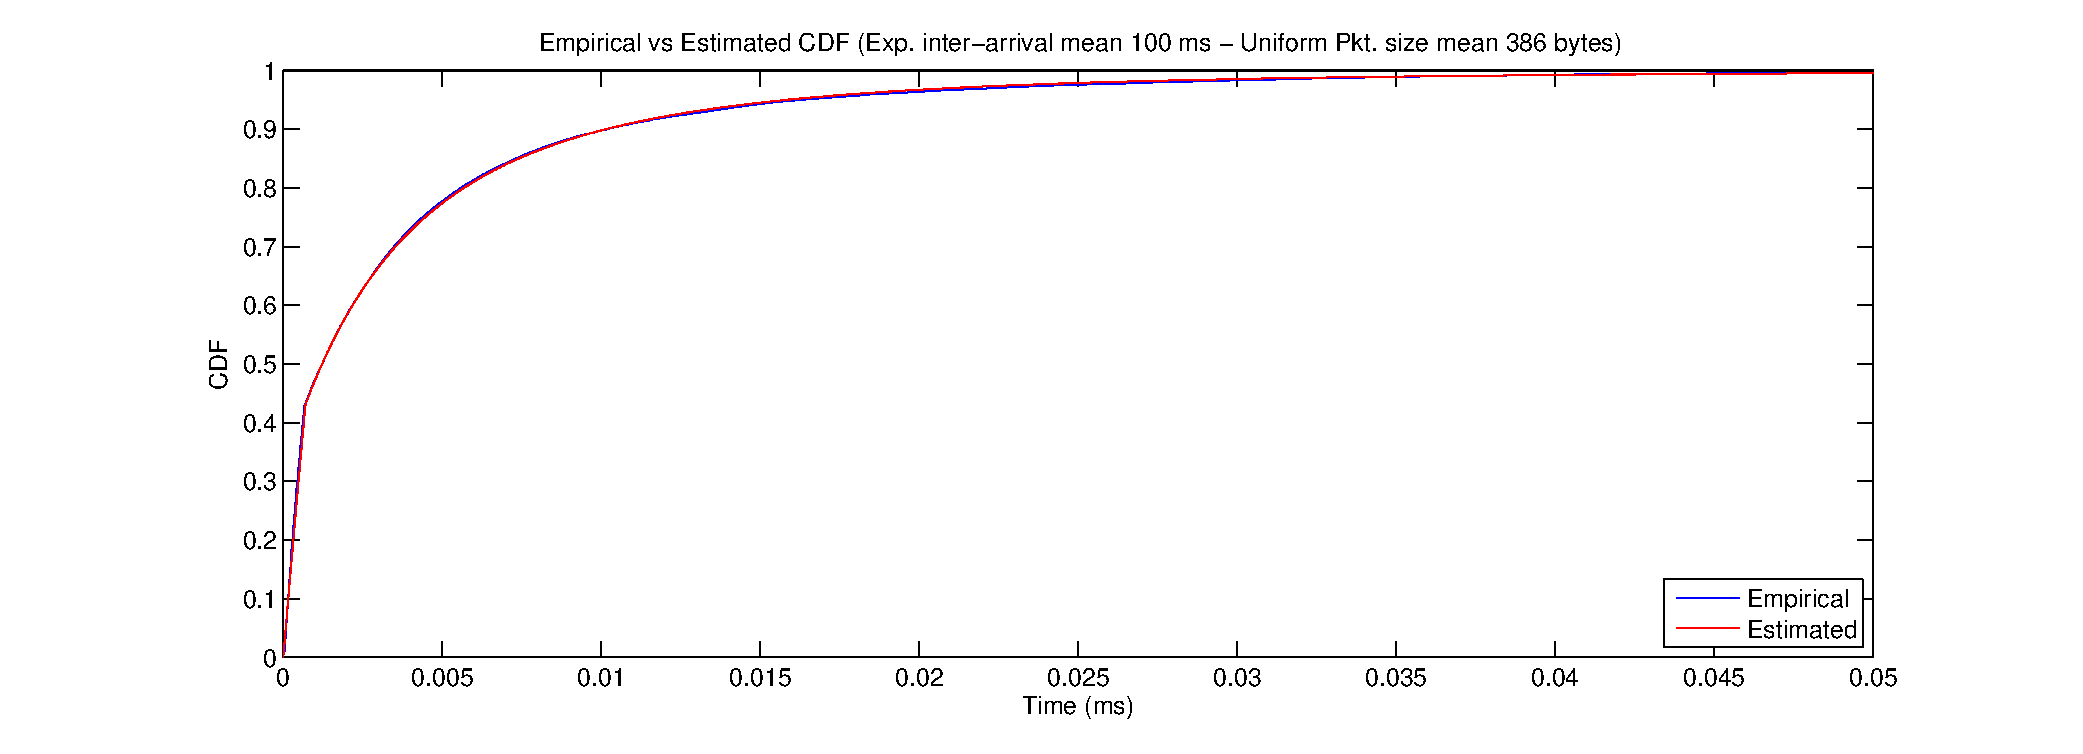
\includegraphics[width=0.9\textwidth, trim = 0mm 0mm 6mm 5mm, clip]{images/results/GlobalView/KS/ks_fail}
	\caption{Perfect fitting of the \acs{CDF} of the experimental and empirical functions for very low p-value.}
	\label{fig:ks_fail}
\end{figure}

\subsubsection{Effect of the number of samples in the Kolmogorov-Smirnov validation test} \label{sec:ks_optimization}
The first implementation of the \acs{K-S} test included a 10 \% of the total idle samples to perform the validation test. The decision of using a percentage of the total number of samples was done just to perform the validation test faster. In this experiment, we tested the performance of the test using all the samples gathered by the sensors and compared against the first implementation in order to observe if a higher number of samples has any impact in the validation test.

We simulated 100 runs of the same traffic configuration for the session and flow levels, randomizing the packet level as it has been done previously following the configuration in Table \ref{table:KS_traffic}.

We compared the results obtained between both \acs{K-S} implementations. The results of this experiment are presented in Figure \ref{fig:ks_optimization}. We represented the CDF of the p-value of the \acs{K-S} for 100 runs of each test and compare the performance of the p-value using different number of samples for the validation test. As it can be observed, the performance of the validation test is highly improved using all the samples for the estimation of the p-value, giving a higher value for the P in the \acs{K-S} test. Table \ref{table:KS_optimized} includes a resume of the three cases under study in Table \ref{table:KS} and compared with the \acs{K-S} performance using all the samples.

\begin{figure}[h!]
	\centering
		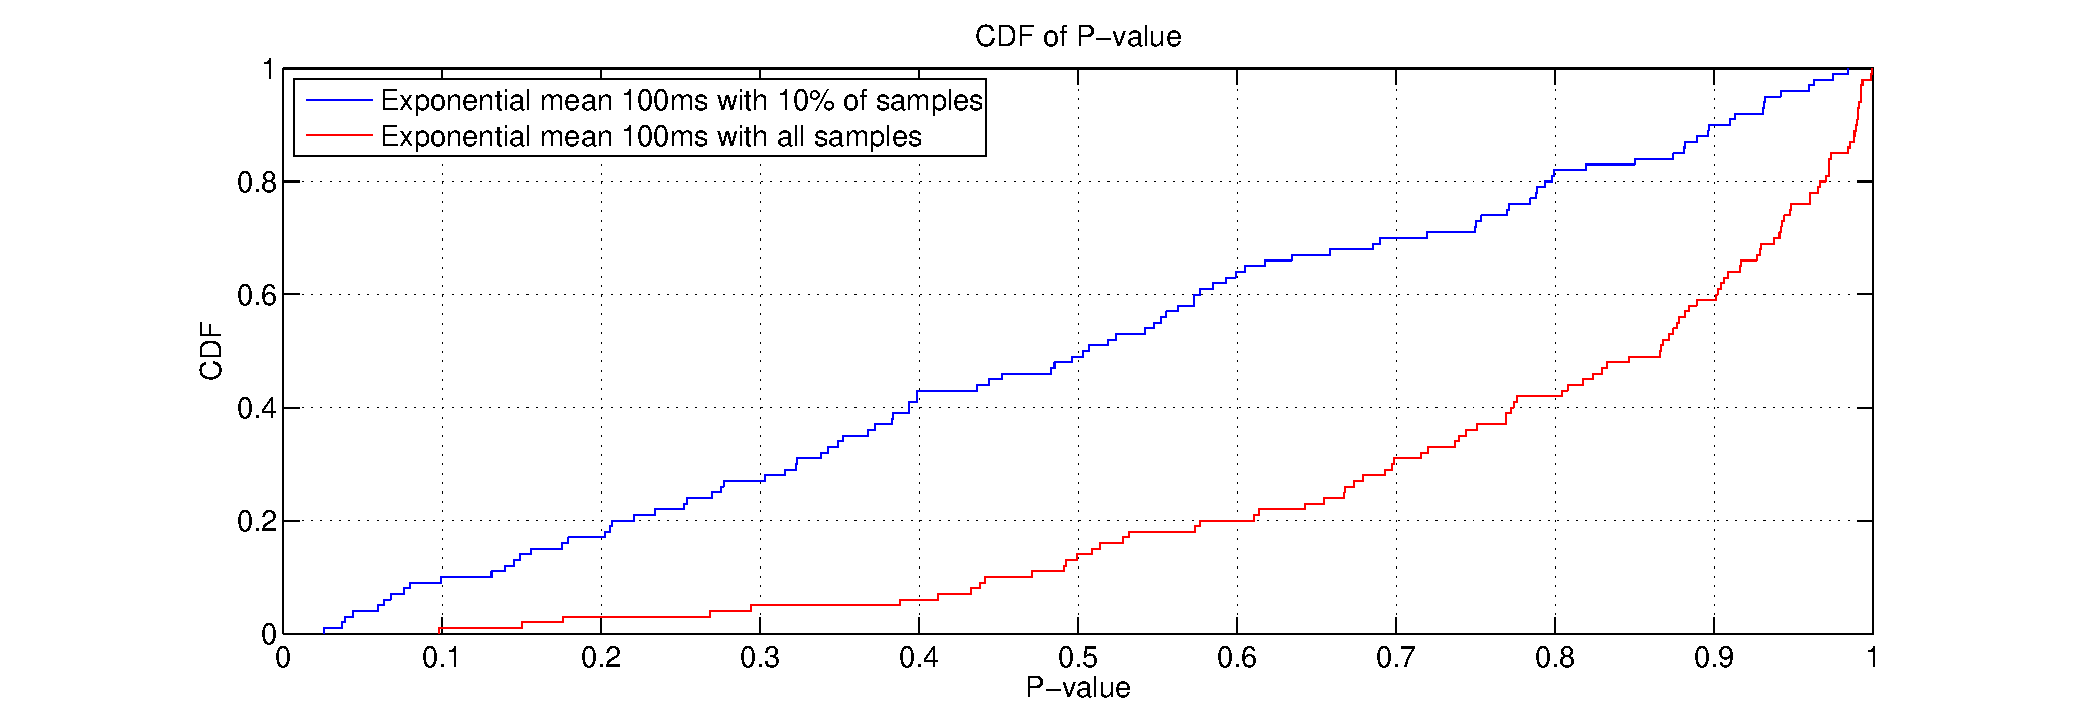
\includegraphics[width=0.9\textwidth, trim = 0mm 0mm 0mm 0mm, clip]{images/results/GlobalView/KS/ks_optimization/pvalue_exponential100ms}
		\label{fig:ks_optimization_exp100}
	\caption{P-value failure rate in the \acs{K-S} test using different number of samples. Exponential packet interarrival with mean 100 ms}
	\label{fig:ks_optimization}
\end{figure}

\begin{table}[h!]
	\centering
	\begin{tabular}{ r | c | c }
		& \acs{K-S} with 10\% of samples & \acs{K-S} with all the samples \\ \hline
		Exponential Interarrival (mean: 1000 ms) & $\approx$ 5.15\% & $\approx$ 0\% \\ 
		Exponential Interarrival (mean: 100 ms) & $\approx$ 4\% & $\approx$ 0\% \\ 
		Uniform Interarrival (mean: 100 ms) & $\approx$ 4.39\% & $\approx$ 3.03\% \\ 
	\end{tabular}
	\caption{\acs{K-S} performance for different packet interarrival distributions and uniform packet size with mean 386 bytes.}
	\label{table:KS_optimized}
\end{table}

As it can be observed from the statistics presented in Table \ref{table:KS_optimized} the failure rate ($P(P-value<0.05)$) is clearly improved, and almost null for the exponential inter-arrival cases under study in Section \ref{sec:ks-results}. On the other hand, that improvement is not that clear for the uniform inter-arrival.

Using a percentage of all the samples for the validation test, it is possible that the firsts and tail samples are excluded from the set of samples that will be used to estimate the p-value of the \acs{K-S} test, affecting the final performance of the validation test. This problem is avoided by using all the set of samples for the validation test and achieving a higher accuracy as it has been demonstrated in this experiment. On the other hand, a higher number of samples implies a higher execution time.

From the results presented in this section, we can conclude that the \acs{K-S} is the correct validation test to be used for our model if all the samples gathered for the estimation of the parameters are also used for the validation test. Using all the idle samples for the validation test we achieve a better performance and avoid the problems presented at the beginning of this section.